\documentclass[12pt]{report}

% Pour le bon support de la langue française : 
\pdfminorversion=5
\pdfobjcompresslevel=2
\usepackage[T1]{fontenc}
\usepackage[utf8]{inputenc}
\usepackage{lmodern}

\usepackage{etex}
\usepackage{lipsum}

% Packages perso :
\usepackage{soul}
\usepackage{fancyhdr}
\usepackage{boxedminipage}
\usepackage{makeidx}
\makeindex
\usepackage{caption}
\usepackage[final]{pdfpages}
\usepackage{listings} % pour inclure des algorithmes
\newcommand{\deriv}{\mathrm{d}}

\usepackage{color} % définit une nouvelle couleur
\usepackage{xcolor}             % Pour mettre de la couleur
% Bibliographie dans la Table des matières
%\usepackage[nottoc, notlof, notlot]{tocbibind} 
\usepackage{authoraftertitle}   %\MyAuthor

\usepackage{float}              % Pour les figures
\usepackage{pgfplots}
\usepackage{tikz}
\usetikzlibrary{arrows,shapes,positioning}
\usetikzlibrary{decorations.markings,decorations.pathmorphing,
decorations.pathreplacing}
\usetikzlibrary{calc,patterns,shapes.geometric}
\tikzset{every picture/.style={execute at begin picture={
\shorthandoff{:;!?};}
}}
\usepackage[europeancurrents,europeanresistors,cuteinductors,europeanports,europeanvoltages]{circuitikz}         % Circuits électriques
\usepackage{thumbpdf}           % Fichier pdf généré 
                                % contien une              
                                % miniature de chaque slide 
%\usepackage{frbib}              % Bibliographie en fr
\usepackage{dashrule}           % Lignes points-tillés
\usepackage{pifont}             % \ding{code utf8}
\usepackage{hyperref}           % Pour ajouter des liens avec \href
\usepackage{lastpage}           % Avoir total de pages dans le footer.
\usepackage{graphicx}           % Pour les images et figures
\usepackage{wrapfig}            % Pour détourer les figures
%\begin{wrapfigure}[lineheight]{alignement}{width}
\usepackage{multicol}           % Doc sur plusieurs colonnes
\setlength{\columnseprule}{.4pt}% Avec séparateur.
\usepackage{fancybox}           % De chouettes encadrements
\usepackage{lettrine}           % Pour de beaux paragraphes
% \usepackage{type1cm}          % scalable fonts pour lettrine
\usepackage{oldgerm}            % Lettrines en gothique
\newcommand{\gothique}[2]{\lettrine{\textgoth #1}{#2}} 
\usepackage{yfonts}             % De belles enluminures
\newcommand{\enluminure}[2]{\lettrine[lines=3]{\small \initfamily #1}{#2}} 
\usepackage{url}                % Pour écrire des url
\usepackage{geometry}
\geometry{margin=60pt}
\usepackage{setspace}           % Pour changer l'interligne
\usepackage{eurosym}            % Pour le signe \euro
\usepackage{colortbl}           % Couleur dans tableaux
\usepackage{tabularx}           % pour des tableaux à taille de la page
\usepackage{longtable}          % Pour les grands tableaux
\usepackage[tight]{shorttoc}    % Pour faire un sommaire à la française.
\newcommand{\sommaire}{\shorttoc{Sommaire}{1}}
\usepackage{array}              % De beaux tableaux
\usepackage{multirow}           % Tableaux sur plusieurs lignes
                                % \multirow{nlignes}{largeur ou *}{contenu}
\usepackage{amsmath}            % Un peu de maths
\usepackage{amssymb}            % Encore des maths
\usepackage{mathtools}
\usepackage{empheq}             % Pour encadrer les équations
\usepackage{pdfpages}           % Pour include des pdf avec
%\includepdf[pages=-]{votre_fichier} 
% ,pagecommand={}               % Pour aussi mettre le num de la page
\usepackage[normalem]{ulem}               % Pour barrer du texte

\usepackage{pgfpages}           % Pour avoir 2 pages sur A4 paysage
\usepackage{datetime}           % Jouer facilement avec les dates
% Pour la physique : 
\usepackage{numprint}           % Pour faire des groupes de 3 nombres
\usepackage[squaren,Gray,cdot]{SIunits} % Unités SI
% Ecrire des symboles atomiques
\newcommand{\noyau}[3]{\prescript{#2}{#3}{\mathrm{#1}}}
% Utilisation $\noyau{C}{12}{6}$

% Pour la chimie : 
\usepackage[version=3]{mhchem}
\usepackage{chemfig}

%%%
% Commandes

% Ajout d'une image avec label
\newcommand{\image}[3]{
% \image{fichier}{label}{description}
\begin{center}
% Nécessite le package float
\begin{figure}[H]
\includegraphics[width=0.8\textwidth]{#1}
\caption{\label{#2}{#3}}
\end{figure}
\end{center}
}

% Ajout d'une image largeur page avec label
\newcommand{\imagebig}[3]{
% \imagebig{fichier}{label}{description}
\begin{center}
% Nécessite le package float
\begin{figure}[H]
\includegraphics[width=1\textwidth]{#1}
\caption{\label{#2}{#3}}
\end{figure}
\end{center}
}

% Une image qui prend toute la page
\newcommand{\imagefull}[1]{
    \newgeometry{margin=0cm}
\begin{center}
\begin{figure}[H]
\includegraphics[width=0.96\paperwidth]{#1}
\end{figure}
\end{center}
\restoregeometry
\nopagebreak
}

% Un encadré grisé
\newcommand{\encadregris}[1]{
\begin{center}
\colorbox{gray!20}{
\begin{minipage}{0.95\textwidth}
{#1}
\end{minipage}
}
\end{center}
}

% Un mot grisé
\newcommand{\motgris}[1]{
\colorbox{gray!20}{{#1}}
}

% Un encadré
\newcommand{\encadre}[1]{
\begin{center}
\fbox{
\begin{minipage}{0.95\textwidth}
{#1}
\end{minipage}
}
\end{center}
}

% flèche
\newcommand{\ra}[0]{
    $\rightarrow$
}

% Image détourée
% \wrapimg{align}{width}{img}
\newcommand{\wrapimg}[3]{
\begin{wrapfigure}{#1}{#2}
\includegraphics[width={#2}]{#3}
\end{wrapfigure}
}

\newcommand{\hdr}[0]{
    \hdashrule{1cm}{1pt}{1pt}
}

\newcommand{\hdrp}[0]{
    \hdashrule{3cm}{1pt}{1pt}
}

\newcommand{\hdrpp}[0]{
    \hdashrule{4cm}{1pt}{1pt}
}

\newcommand*{\etoile}
{
\begin{center}
*\par
*\hspace*{3ex}*
\end{center}
}

% petit carré
\newcommand{\petitcarre}{\rule[.2ex]{0.75ex}{0.75ex}}

%incertitude relative
\newcommand{\incertRel}[1]{
    \frac{\Delta {#1}}{{#1}}
}

% listes avec puces carrées
\newcommand{\carlst}[1]{
    \begin{itemize}
    \renewcommand\labelitemi{\petitcarre}
    {#1}
    \end{itemize}
}

% \emph plus simple
\newcommand{\e}[1]{\emph{{#1}}}

% equation encadrée
\newcommand{\boxeq}[1]{
    \begin{empheq}[box=\shadowbox]{align}
    {#1}
    \end{empheq}
}

%%% Schémas de chimie %%%

% Schema de titrage
% \schemaTitrage{solution titrante}{solution titrée}
\newcommand{\schemaTitrage}[2]{
    \begin{tikzpicture}
        \draw [thick]
        (0,0) -- ++ (2,0) -- ++ (0,1) -- ++ (-2,0) -- ++ (0,-1)
        (0.3,3) -- ++ (0,-2)
        (1.7,3) -- ++ (0,-2)
        (1,6) -- ++ (0,-3)
        (0.8,3.3) -- ++ (0.4,0)
        (0.3,1.7) -- ++ (1.4,0)
        (0.3,0.3) circle(0.1)
        (1,1.11)ellipse (0.25 and 0.10) 
        ;
        \draw
        [<-,>=stealth] (1,4.4) -- ++ (1.5,0) node[right]  {
            \begin{minipage}{0.275\textwidth}
                {#1}
            \end{minipage}
        }
        ;
        \draw
        [<-,>=stealth] (1,1.5) -- ++ (1.5,0) node[right] {
            \begin{minipage}{0.27\textwidth} 
            {#2}
            \end{minipage}
        }
        ;
    \end{tikzpicture}
}

% Tube à essai légendé.
\newcommand{\schemaTubeEssai}[1]{
    \begin{tikzpicture}[scale=0.25]
    \draw
    (0,0) arc (0:-180:1)
    (-2,0) -- ++ (0,8)
    (0,0) -- ++ (0,8)
    (-2,4) -- ++ (2,0)
    (-0.5,-1) node[below] 
        {
        \begin{minipage}{0.2\textwidth}
        {#1}
        \end{minipage}
        }
    ;
    \end{tikzpicture}
}
% Papier millimétré
% \papmili{x}{y}
\newcommand{\papmili}[2]{
\begin{tikzpicture}
\draw[step=1mm, line width=0.1mm, black!30!white] (0,0) grid
({#1},{#2});
\draw[step=5mm, line width=0.2mm, black!40!white] (0,0) grid
({#1},{#2});
\draw[step=5cm, line width=0.5mm, black!50!white] (0,0) grid
({#1},{#2});
\draw[step=1cm, line width=0.3mm, black!90!white] (0,0) grid
({#1},{#2});
\end{tikzpicture}
}
% \grap{x}{y}{legende x}{legende y}
\newcommand{\graph}[4]{
\begin{tikzpicture}
\draw[step=1mm, line width=0.1mm, black!30!white] (0,0) grid
({#1},{#2});
\draw[step=5mm, line width=0.2mm, black!60!white] (0,0) grid
({#1},{#2});
\draw[step=5cm, line width=0.5mm, black!80!white] (0,0) grid
({#1},{#2});
\draw[line width=0.6mm, ->, >=stealth] (0,0) -- ({#1},0)
node[right]{{#3}};
\draw[line width=0.6mm, ->, >=stealth] (0,0) -- (0,{#2})
node[above]{{#4}};
\end{tikzpicture}
}

\usepackage{listingsutf8}

\lstdefinestyle{customc}{
  belowcaptionskip=1\baselineskip,
  breaklines=true,
  frame=L,
  xleftmargin=\parindent,
  language=C,
  showstringspaces=false,
  basicstyle=\footnotesize\ttfamily,
  keywordstyle=\bfseries\color{green!40!black},
  commentstyle=\itshape\color{purple!40!black},
  identifierstyle=\color{blue},
  stringstyle=\color{orange},
}

\lstdefinestyle{customasm}{
  belowcaptionskip=1\baselineskip,
  frame=L,
  xleftmargin=\parindent,
  language=[x86masm]Assembler,
  basicstyle=\footnotesize\ttfamily,
  commentstyle=\itshape\color{purple!40!black},
}

\lstset{escapechar=@,style=customc}

\pagestyle{fancy}
\fancyhead[L]{}
\fancyhead[R]{}
\fancyfoot[L]{}
\fancyfoot[R]{}


\begin{document}

\newlength{\larg}
\setlength{\larg}{14.5cm}
\lstset{inputencoding=utf8/latin1}
\title{
{\rule{\larg}{1mm}}\vspace{7mm}
\begin{tabular}{p{0cm} c}
   & { {\textbf{Tutorial}}} \\
   & {\huge Use anatomical mesh classes.} \\
\end{tabular}\\
\vspace{2mm}
{\rule{\larg}{1mm}}
\vspace{2mm} \\
\begin{tabular}{p{11cm} r}
   & {\large  25/08/2016}
\end{tabular}\\
\vspace{2cm}
\large{\textit{} \\
BANGOR UNIVERSITY\\
School of Computer Science}
\vspace{5cm}
}
\author{\begin{tabular}{p{13.7cm} r}
Andréas MEULEMAN
\end{tabular}\\
\hline }
\date{}
\maketitle

\chapter{Introduction}

	The complete source code of this tutorial is available on the Subversion (SVN) repository at $tutorials/tutorial\_04\_qt4$. 
	
	$AnatomicalMesh$ is a virtual class inheriting from PolygonMesh\footnote{Class diagram in annexe.}. It was made to hadle meshes for different tussies. Five classes are inheriting from $AnatomicalMesh$: $SkinMesh$, $LungsMesh$, $LiverMesh$, $DiaphragmMesh$ and $BoneMesh$. They are all implementing the following public functions: \\ 

\begin{lstlisting}
	/// return true if the mesh has to be displayed with transparency
	bool isTransparent() const;

	/// return true if the mesh represent a soft tissue
	bool isSoftTissue() const;

	/// Link the attributes to their id in the shader
    	/// shader_id: The GLSL shader used to display the anatomical mesh
	void defineDisplayShaderInput(int shader_id);

	/// initialize the shaders, the buffers, the normal vectors and the textures
	void initialize();
\end{lstlisting}
~\\

	$SkinMesh$ is transparent and white by default.The other classes generate suitable textures and normal maps. They are procedural generated using noise so that they are slightly different after each launch of the program. These classes are supposed to be used with the shaders $display\_realistic\_gl3.vert$ and $display\_realistic\_gl3.frag$. 

	To use these classes, we need to set the data (vertices position and normal vectors) as we do for any PolygonMesh and then, call $defineDisplayShaderInput(int$ $shader\_id)$ just before the polygonMesh's function $display()$. In this tutorial, we will display lungs without lighting.
	
\newpage

	Here is an example of rendering using some of these classes: \\
	
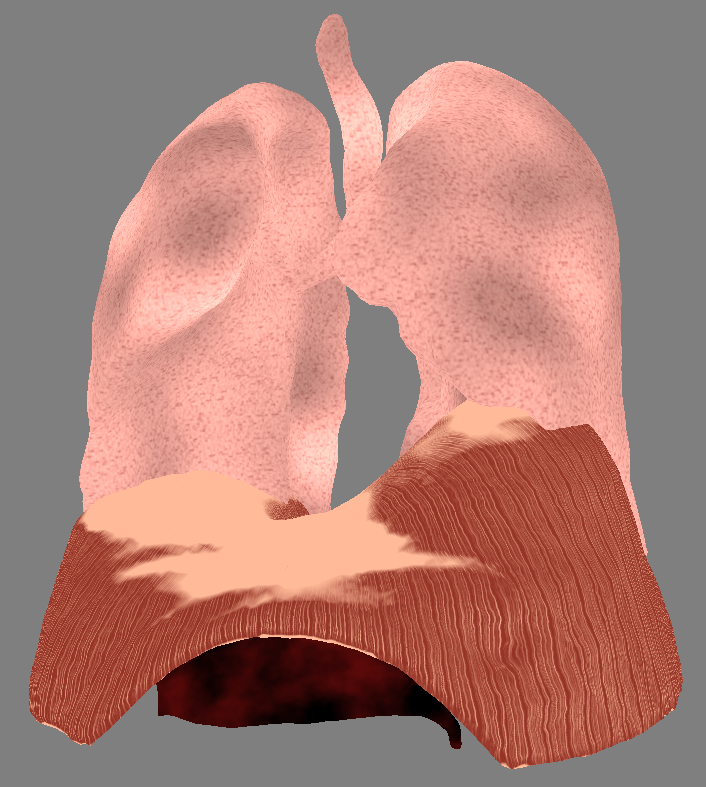
\includegraphics[scale = 0.6]{img/AllMeshes.png}


\chapter{includes}

These are to use the shaders $display\_realistic\_gl3.vert$ and $display\_realistic\_gl3.frag$:
\begin{lstlisting}
#include "display_realistic_gl3.frag.h"
#include "display_realistic_gl3.vert.h"

#ifndef GVXR_MATRIX4X4_H
#include "gVirtualXRay/Matrix4x4.h"
#endif

#ifndef GVXR_SHADER_H
#include "gVirtualXRay/Shader.h"
#endif
\end{lstlisting}

We have to include the header of the class we are going to use:
\begin{lstlisting}
#include "gVirtualXRay/LungsMesh.h"
\end{lstlisting}

\chapter{Build the objects}

	the constructor of all the classes inherating from $InternalOrganMesh$ ($LungsMesh$, $LiverMesh$, $DiaphragmMesh$ and $BoneMesh$) have parameters to control the texture generation. 
	
	$LungsMesh$, $LiverMesh$ and $DiaphragmMesh$ use 2D texturing. $texture\_2D\_size$ represent the size in pixels of the side of the 2D textures used for this mesh. Its default value is 2048 for the lungs and the diaphragm and 512 for the liver but it can be modified depending on the graphic card's amount of vram.
	
	These constructors have a $bool$ parameter $optimize_texture_coordinates$. If it is true, the 2D texture coordinates will be optimize before the rendering. Optimize the texture coordinates enable a better rendering with the same performances, but it requires more precomputating. Its default value is true. \\
	
	$BoneMesh$, $LiverMesh$ and $LungsMesh$ use 3D texturing, the $unsigned$ $int$ parameter $texture\_3D\_size$ of their constructors is the size of the side of the 3D texture. Its default value is $32$, 3D textures have to be small since they use a lot of vram.
		
	The constructor of $LungsMesh$ has three other parameters of type $bool$: $x\_mirror$, $y\_mirror$ and $z\_mirror$. They enable to know if the mesh is upside down to draw the lines correctly. Their default value is false.

	The constructor of $SkinMesh$ has no parameters.

\chapter{Load the data}

To load the vertices data of the anatomical mesh, we can use any of the techniques for polygon meshes shown in the previous tutorials. When a textured anatomical mesh is used, the index of the mesh is remove before generating the textures.

	We have to be carefull with that if the data loaded involve indices and make sure that the index isn't built again. In case the index is built again, the index can be removed again by calling the function $initialize()$, but it require some computating from the cpu.

\chapter{Display the organ using OpenGL}

To use this shader program without lighting, we have to define the projection matrix, the modelview matrix and a flag to avoid using lighting:

\begin{lstlisting}
        // Handle for shader variables
    	GLuint handle(0);

    	handle = glGetUniformLocation(shader_id, "g_projection_matrix");
        glUniformMatrix4fv(handle, 1, GL_FALSE, g_current_projection_matrix.get());
        checkOpenGLErrorStatus(__FILE__, __FUNCTION__, __LINE__);

        handle = glGetUniformLocation(shader_id, "g_modelview_matrix");
        glUniformMatrix4fv(handle, 1, GL_FALSE, g_current_modelview_matrix.get());
        checkOpenGLErrorStatus(__FILE__, __FUNCTION__, __LINE__);

        //Don't use lighting
        GLint lighting;
        lighting = 0;
        handle = glGetUniformLocation(shader_id,"g_use_lighting");
        glUniform1iv(handle, 1, &lighting);
        checkOpenGLErrorStatus(__FILE__, __FUNCTION__, __LINE__);
\end{lstlisting}

Then we use the function of the lung mesh to define the others inputs:

\begin{lstlisting}
        m_lung_mesh.defineDisplayShaderInput(shader_id);
\end{lstlisting}

Finally, we can display the mesh:

\begin{lstlisting}
        // Display the current patient
   		m_lung_mesh.display();
\end{lstlisting}

\chapter{result}

The lungs is automatically textured:\\

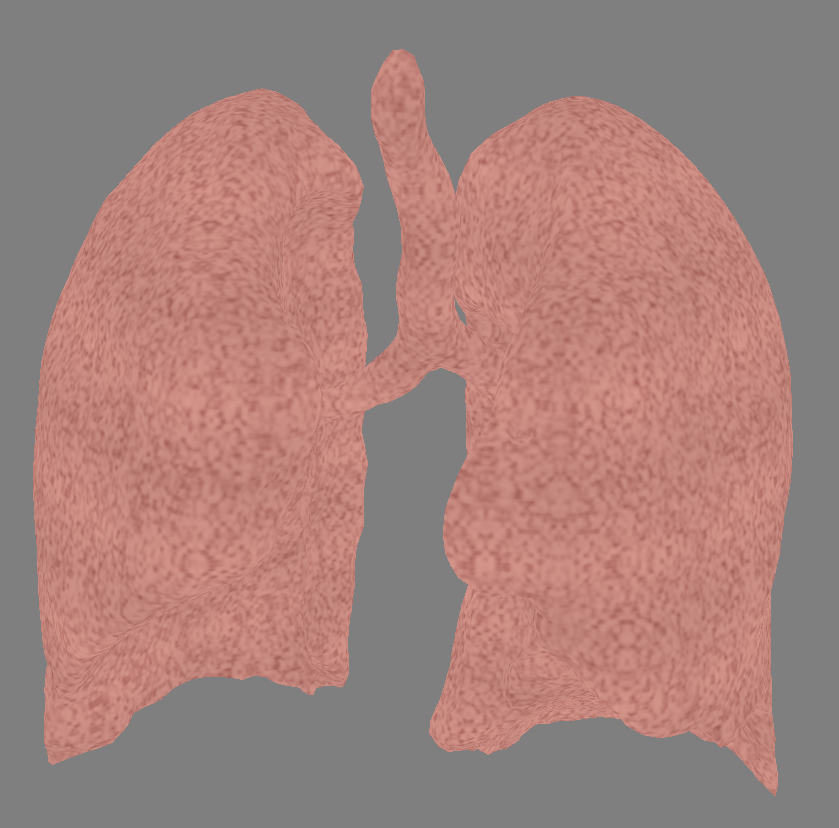
\includegraphics[scale = 0.5]{img/textured_lungs.png}

\chapter{Annexe}

The class diagram of the anatomical mesh classes:\\

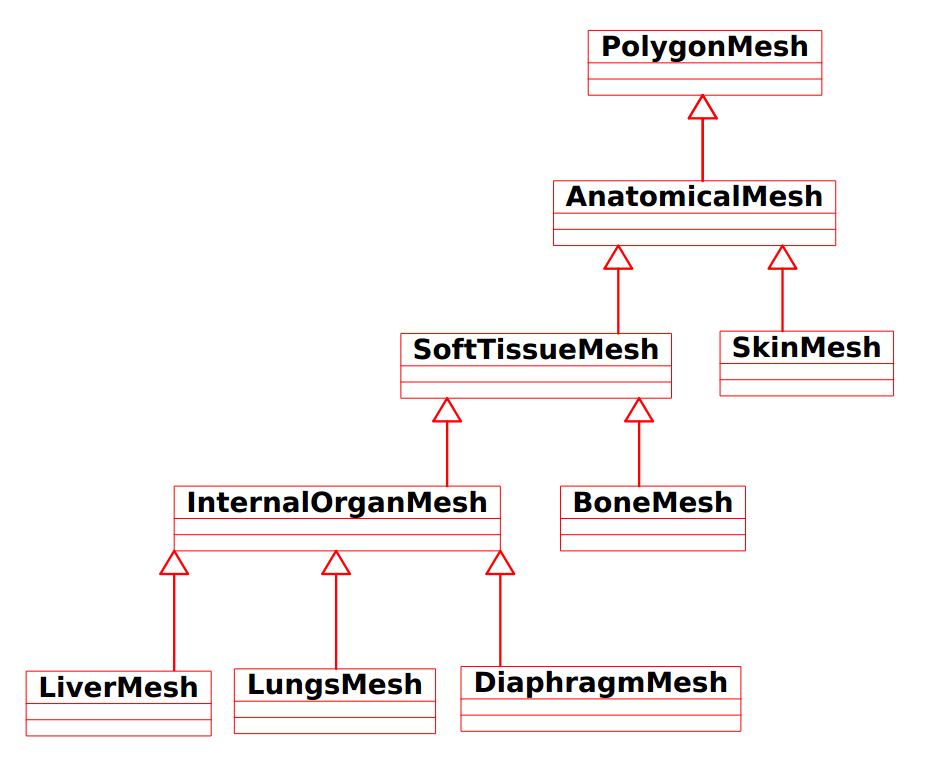
\includegraphics[scale = 0.5]{img/UML.png}

\end{document}